\section{Les bas fonds de Taris} \label{sec:sc2-taris}

C’est parti pour le deuxième volet de la campagne. C’est un épisode qui peut, selon les choix des héros, être assez long. L’épisode précédent était d’environ deux heures, cet épisode peut durer jusqu’à 4 heures selon les directions prises. Il peut aussi être beaucoup plus court si les héros empruntent tous les raccourcis. C’est a vous de doser les ennemis et les choix pour adapter le temps de jeu à ce que vous souhaitez.

\subsection{Prologue}
Nos héros se retrouvent donc dans un Cargo léger YZ-775 sans canons fonctionnels et un message entrant d’une inconnue qui demande à parler à Tinon.
    
Ils ont aussi appris qu’Industrial Automaton sous couvert d’expérimentations de son nouveau modèle, fait des recherches sur un très ancien artefact Sith en provenance de \textbf{Taris}. De plus, s’ils ont réussi à récupérer le droïde, Vyna Anen les attend sur l’avant-poste commercial de \textbf{l’anneau de Kafrene} au Starlord Café. Enfin, ils savent aussi que le vaisseau se dirigeait vers \textbf{Gaulus} pour rejoindre un laboratoire de l’empire où il devait finir des recherches sur l’artefact.

Plusieurs directions s’offrent alors à nos héros.

\subsection{Les bons, les brutes ou les truants}
\begin{quotebox}
    Tinon \emph{(prononcer Taïnon)} c’est toi ? Que se passe t’il ou va tu ?
\end{quotebox}
Le visage d’une jeune femme apparaît sur l’holocomm. Les héros ont le choix de répondre ou non.

Ce point de l’aventure est crucial pour nos héros car ils vont choisir (en connaissance de cause ou non) l’orientation de leurs personnages. En effet plusieurs cas de figures se présentent :

\begin{description}
    \item[\nameref{sec:les-rebelles}] Répondre au message et suivre les consignes des Rebelles (page~\pageref{sec:les-rebelles}).
    \item[\nameref{sec:retour-du-droide}] Ramener le droïde à Vyna Anen (page~\pageref{sec:retour-du-droide}).
    \item[\nameref{sec:refus-d-obtemperer}] Partir pour Taris directement (page~\pageref{sec:refus-d-obtemperer}).
    \item[\nameref{sec:l-empire}] Prendre la direction de Gaulus (page~\pageref{sec:l-empire}).
\end{description}

Tous ses choix amèneront, de toute façon, les héros sur Taris mais le chemin sera différent et par là même leur orientation aussi. Je vais tâcher de décrire les choix possibles sachant que rien n’est écrit dans le marbre et vous pouvez très bien les forcer suivre une route en particulier. C’est un peu le jeu de piste, les choix s’entrecroisent alors faut suivre. Mais une fois de plus rien n’est définitif, les joueurs auront toujours des idées farfelues auxquelles on n’a pas pensé mais je vais essayer de décrire les principales voies possibles, au MJ de diriger les joueurs vers une de ces voies.


\subsubsection{Retour du droïde} \label{sec:retour-du-droide}

Autre choix possible pour les héros, ces derniers, avides de crédits, veulent aller rendre le droïde et récupérer le solde promis pour leur mission. Ils retournent donc sur l’avant-poste commercial dans \textbf{l’anneau de Kafrène} où les attend \nameref{sec:vyna-anen}.

On laisse les héros discuter un peu et réclamer leur due, Vyna acquiesce avec le sourire, leur donne les crédits mais au moment de quitter la pièce, 4 ou 5 \textit{(doser en fonction du niveau de vos joueurs)} Stormtroopers leur barre la route. Attention, à moins que les héros aient anticipé, le premier tour de combat sera pour dégainer.

\begin{quotebox}
    Vous pensiez réellement qu’avec tout ce que vous savez, nous allons vous laisser repartir tranquillement ?\\
    Commencez par me rendre les crédits.
\end{quotebox}

Les héros peuvent tenter de négocier avec Vyna, ce dernier acceptera de les laisser repartir vivant (mais sans crédit) à condition qu’ils retournent sur \nameref{sec:taris} et récupèrent les informations que les scientifiques de Industrial Automaton n’ont pas eu le temps de récupérer. Ils peuvent tenter un jet de Persuasion pour garder les crédits.\\

Si les héros entrent en combat, et qu’ils perdent, on ne les tue pas mais Vyna leur impose de retourner sur Taris et pas de négociation possible. S’ils gagnent, deux cas de figure possibles :
\begin{rebelist}
    \item \textbf{Ils tuent Vyna} Un homme, Chiss, manifestement important en uniforme de l’empire entre dans la pièce en applaudissant. Posément, il félicite les joueurs et leur explique qu’ils ont réussi le test avec brillo. Vyna était devenu gênant pour l’empire et pour l’Odre. Si l’un des héros tente quoi que ce soit il se retrouve désarmé et collé au mur avant d’avoir eu le temps de comprendre. On décroche sur \nameref{sec:l-empire}.

    \item \textbf{Ils laissent Vyna en vie} Une femme (celle qui est apparue sur le holocom du vaisseau) entre dans la pièce avec deux hommes. Les deux hommes emportent Vyna avec eux, en faisant comme s’il était ivre. Et la femme leur fait signe de la suivre vite, elle leur expliquera plus tard. Ils prennent le vaisseau et partent pour la cache des Rebelles. On décroche sur \nameref{sec:les-rebelles} dans la version bien accueillie.
\end{rebelist}

Le \nameref{sec:nimbus} n’est réparé qu’à leur demande, le prix est de 40~000 \crg. Négociable (Persuasion) à 30~000, -10k si relance.


\subsubsection{Les rebelles} \label{sec:les-rebelles}

\begin{quotebox}
    Tinon \emph{(prononcer Taïnon)} c’est toi ? Que se passe t’il où va tu ?
\end{quotebox}

Le visage d’une jeune femme apparaît sur l’holocomm et les héros choisissent de répondre.

\begin{quotebox}
    Mais qui êtes vous et où et Tinon ?
\end{quotebox}
Les joueurs choisissent de raconter leur histoire, ou de mentir, à voir ce qu’ils préfèrent. Lindi leur demande de la rejoindre et leur donne les coordonnées d’une cache de la Rébellion. Si les joueurs ont menti, ils sont accueillis avec suspicion, menacé et tout ce qui va avec, sinon ils sont accueillis normalement avec juste un peu de méfiance. \nameref{sec:lindi-dangon} les invite à la suivre et les interroge jusqu’à ce qu’ils disent la vérité (On part du principe que s’ils persistent à mentir, on bifurque vers l’option \nameref{sec:refus-d-obtemperer}).

Lindi leur explique alors que la résistance a eu vent des recherches menées par l’Industrial Automaton ainsi que des problèmes sur le Pelican. \textbf{Tinon Dystra} avait été envoyé pour tenter de s’infiltrer à bord du Pelican. Mais qu’il n’avait plus donné de nouvelles depuis son arrimage au vaisseau.

Un jet de \textbf{Perception} ou l’utilisation de \textbf{Sens de Force} fera apparaître les sentiments de Lindi envers Tinon et apprendra à nos héros que ces derniers étaient amants.\\

Une fois la discussion terminée, Lindi demande de l’aide aux héros, qu’ils reprennent le travail de Tinon. La première piste à explorer étant \ldots \nameref{sec:taris}.

Le \nameref{sec:nimbus} est réparé gratuitement pendant que les héros discutent.


\subsubsection{Refus d’obtempérer} \label{sec:refus-d-obtemperer}

Les héros veulent se la jouer et décident de partir direct sur Taris. Mais ils ne savent même pas trop ce qu’ils y cherchent. L’hyper-espace est récalcitrant et ne veut pas fonctionner immédiatement. Le temps de regarder, un croiseur sort d’hyper-espace et les arraisonne sans poser de questions. Des soldats de l’alliance (trop pour être combattu) forcent la cloison et entrent dans le cargo, suivis par la femme vue précédemment sur l’holocomm.

\begin{quotebox}
    Où pensiez-vous partir comme ça avec ce cargo ? \\
    \emph{se retournant vers les soldats}, jetez-moi ça en cellule on les interrogera là-bas.
\end{quotebox}

Les héros sont transportés jusqu’à une cache de la Rébellion et jetés en cellule. Au bout de quelque temps, la femme précédemment rencontrée vient les interroger. Ils ont le choix de répondre la vérité ou de mentir. S’ils répondent la vérité, on décroche sur l’option correspondante dans \nameref{sec:les-rebelles}. Sinon ils sont laissés en cellule \ldots

Mais dans la nuit, un mystérieux inconnu s’approche de la cellule sans bruit

\begin{quotebox}
    Je suis envoyé par Vyna Anen, si vous voulez vivre, venez avec moi et pas un bruit.
\end{quotebox}

L’inconnu ouvre leur cellule et les emmène au cargo. Sur le chemin, leur demander des jets de \textbf{Discrétion}. En cas d’échec deux soldats débarquent. Dans le hangar où se trouve le cargo, 4 soldats montent la garde. Soient les héros passent en force et débutent un combat puis vont ouvrir les portes du hangar. Soit ils la jouent furtif, se glissent dans le vaisseau et tirent sur les portes pour sortir du hangar. Ou n’importe quoi d’autres qui leur permet de sortir. Une fois dehors l’inconnu leur transmet des coordonnées. Ils n’ont pas le choix, s’ils font mine de résister, l’inconnu sort une arme et les tiens en joue. Eux n’ont pas d’arme ils sortent de cellule. On décroche ensuite sur \nameref{sec:l-empire}.



\subsubsection{L’empire} \label{sec:l-empire}
Enfin, dernière alternative les héros peuvent vouloir partir pour \textbf{Gaulus} la planète vers laquelle se dirigeait le vaisseau. 

\'A l’approche de la planète, le cargo est arraisonné par un croiseur de l’empire. Les héros sont invités à sortir et une dizaine de Stormtroper les attendent. Ils sont escortés jusque dans un bureau où les attendant \nameref{sec:vyna-anen} et un Chiss en uniforme de gradé de l’empire. C’est ce dernier qui prend la parole.

\begin{quotebox}
    Messieurs (mes dames) nous vous attendions. Asseyez-vous je vous pris. \\
    Alors comment s’est passé cette mission, je vois que tout le monde n’est pas revenu \emph{(sourire aux lèvres)}. 
\end{quotebox}

Le droïde est emmené par deux gardes. Puis le Chiss se présente.

\begin{quotebox}
    Je me présente, je m’appelle \nameref{sec:garan-keggle}, j’ai suivi la mission de loin et je tiens à vous féliciter, vous vous en êtes sorti plutôt bien. Je pensais pas que vous viendriez à bout de l’Amblyope mais j’avoue que le combat était intéressant. Au vu de vos qualités respectives, je souhaiterais que vous partiez pour \nameref{sec:taris} afin de finir la travail \emph{(il jette un regard froid sur Vyna qui en même pas large et baisse les yeux)} nous avons besoin de plus d’information sur la position de l’artéfact.
\end{quotebox}

Si les héros se hasardent à demander un prime, on leur répond que l’empire saura les récompenser sans plus de détail. S’ils sont récalcitrants, on leur explique que c’est pas une proposition que l’on vient de leur faire.


\subsection{Taris} \label{sec:taris}
\noindent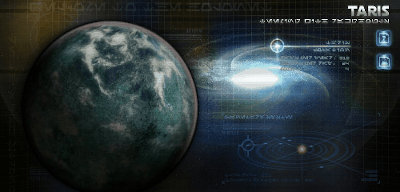
\includegraphics[width=\linewidth]{_img/places/taris.jpg}
Taris est une planète urbaine, très polluée, de la Bordure Extérieure. Divisée en trois grandes parties en fonction des étages, la Ville Haute, la ville basse et les “bas fonds”, elle abritait autrefois une population gigantesque. Grand pôle économique dans la galaxie, notamment grâce à l’implantation des industries Lhosan, elle joignit la République Galactique peu avant les Guerres Mandaloriennes. Mais après le passage de Dark Malak plus de 4000 ans auparavant la planète a du mal à reprendre vie. Les "bas fonds", qui abritaient toutes sortes de hors-la-loi et de rebus de la société, est la partie de Taris qui s’en est le mieux sortie et c’est pourquoi les ruines marécageuses de Taris sont très dangereuses. La république a depuis implanté un spatioport et une base militaire sur la planète dans l’espoir de la recoloniser mais le processus s’avère lent et compliqué.

Normalement une fois au spatioport, vos héros ne savent pas où aller. Plusieurs choix s’offrent à vous pour les orienter, comme de leur placer un bar bien en évidence sur leur chemin. \'A l’intérieur ils pourront trouver des informations et peut-être même un guide.

Normalement, ils vont se diriger vers le barman. Au pire, c’est le barman qui vient à eux pour leur demander ce qu’ils veulent boire. Ce dernier, un Besalisk, leur explique que l’endroit où ils souhaitent se rendre (les ruines de l’ancien temple Sith) se trouve dans un zone interdite, au c\oe{ur} de la zone de quarantaine \nameref{sec:rakghoul}. Il n’est pas possible de s’y rendre.

Mais un client du bar les accoste et leur dit que moyennant 20~000 \crg il les conduira où ils le souhaitent. Un jet de Persuasion (opposé à la Persuasion de l’inconnu 5) fera descendre la somme à 15~000 \crg.

\begin{paperbox}{Quête annexe (optionnel)}
    Il est possible d’intégrer une petite quête annexe ici histoire de varier les plaisirs. S’ils la réussissent on pourra distribuer +1 XP supplémentaire.

    L’inconnu propose à vos héros de les conduire gratuitement aux ruines s’ils l’aident. Selon l’orientation des joueurs à ce moment, soit:
    \begin{description}
        \item [obscur] Ils aident un contrebandier à Kidnapper une jeune Twi’lek repérée dans un camp de réfigiés pas loin.
        \item [clair] Ils aident un père à délivrer sa fille (adoptive) Twi’lek des mains de contrebandiers.
    \end{description}

    Le roleplay est un peu différent selon la situation mais la quête se déroule de la même façon. Les héros suivent l’inconnu qui s’est présenté entre-temps (\nameref{sec:gil-harend}). Ce dernier les conduit au camp (de réfugiés ou de contrebandier). Un jet de Discrétion réussi par tout le monde permet de s’approcher de la cible. Un jet de discrétion réussi par tous permet de s’extraire de camp sans encombre. Le joueur qui est chargé de transporter la cible à un malus de -2 à son deuxième jet de discrétion.

    Si une Discrétion est ratée par l’un des joueurs, un combat commence. Vos héros se trouve confronté à H -1 contrebandiers/réfugiés (H est le nombre de joueurs que vous avez). Vos héros ont l’initiative sur le premier round. En face, les ennemis ont les caractéristiques \nameref{sec:taris-contrebandier}.

    Attention, \nameref{sec:gil-harend} ne doit pas mourir sinon la quête est un échec et retour au bar. 
\end{paperbox}

\begin{paperbox}{Les aléas du direct}
    Lors du scénar, le droïde était avec les joueurs. Ce dernier connaissait donc les coordonnées des ruines Sith. Il ne leur restait qu’à trouver une guide pour passer les barrages de la zone de quarantaine. L’un des joueurs avec l’Atout \textit{Réseaux} et a souhaité l’utiliser et a fait un jet assez magistral. \nameref{sec:gil-harend} s’est donc trouvé être un ancien camarade du joueur et la quête s’est poursuivie sur cette base.
\end{paperbox}

\subsubsection{Les ruines de l’ancien temple Sith}
\noindent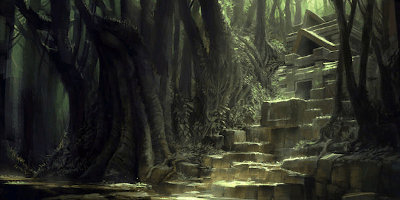
\includegraphics[width=\linewidth]{_img/places/taris-temple-sith.jpg}

Après plusieurs heures de marche dans les marécages de Taris, le groupe arriver devant les ruines de l’ancien Temple Sith. Le côté obscur de la Force émane du temple dans toutes les directions et l’atmosphère est pesante. D’ailleurs on entend absolument aucun bruit, comme si toute la faune avait déserté la zone. L’entrée est partiellement éboulée mais il reste une ouverture suffisante pour s’y faufiler.

Après être entré dans le temple les héros se retrouvent dans une immense salle, très haute de plafond. Deux rangées de statues de 10m de haut représentent d’anciens seigneurs Sith (Un jet de Connaissance (Sith) permet d’apprendre qu’il s’agit de Tulak Hord, Dakhan Shar, Naga Sadow, \ldots entre autres). Au fond de la salle une fresque murale est gravée sur un monolithe.

Chacun des murs de la pièce (en dehors de celui de l’entrée dans leur dos) possède deux ouvertures vers des pièces.

Devant le monolithe, les vestiges d’un campement de fortune (attention, c’est des vestiges de 3000 ans quand même, heureusement à l’époque on faisait les choses pour que ça dure ;-) ) recouvert de poussière. Une partie de ce campement semble pourtant avoir été remué récemment.

Naturellement, nos héros ne sont pas seuls. 5 \nameref{sec:rakghoul} débarquent et encerclent les héros, s’ensuit une phase de combat.
\\

Une fois les Rakghouls éliminés, les héros peuvent aller observer le monolithe et le campement.
\\

Un jet de \textit{Connaissance (Sith)} permet de comprendre la fresque. Avec une relance, le héros remarquera un étrange renfoncement dans le Monolithe, en forme de triangle.

S’ils ne font pas ce jet ou qu’ils le ratent, ils ne peuvent que tenter d’interpréter la fresque. Après il leur est possible de faire des recherches sur cette fresque dans un temple Jedi ou une bibliothèque. En soi l’histoire n’a pas une grosse importance pour la suite, c’est un bonus pour eux.
\\

\textit{La version intégrale de la fresque, sans les explications est présente dans le répertoire "\_img/places/monolithe.jpg" du dossier}

\clearpage

\begin{quotebox}
\noindent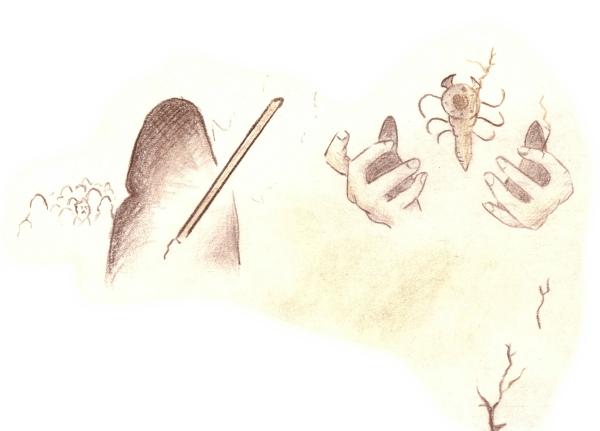
\includegraphics[width=\linewidth]{_img/places/monolithe-001.png}
6000 ans par le passé, un Jedi fut exilé pour ses penchants obscurs et ses expériences interdites sur la vie. Son objectif était, en utilisant le côté obscur, de pouvoir plier la vie elle-même à sa volonté et ainsi acquérir la vie éternelle. En étudiant l’alchimie du côté obscur il parvient à créer un Talisman renfermant son essence et sa volonté. 

\noindent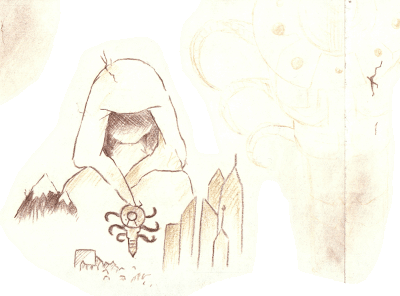
\includegraphics[width=\linewidth]{_img/places/monolithe-002.png}

Cet artefact devait, entre autres, lui permettre de prendre possession du corps du porteur du Talisman mais aussi de contrôler les Rakghoul.

\noindent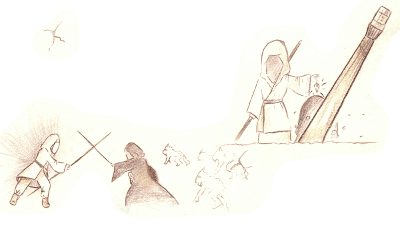
\includegraphics[width=\linewidth]{_img/places/monolithe-003.png}

Ce Jedi Noir fut tué par un de ses rivaux et durant les décennies suivantes plusieurs Seigneurs Sith se déchirèrent entre eux afin de mettre la main sur ce Talisman. 

\noindent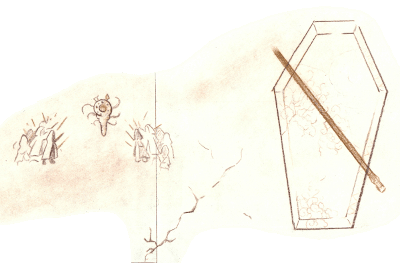
\includegraphics[width=\linewidth]{_img/places/monolithe-004.png}

Enfin, l’artefact et son porteur du moment finirent par être tué et enseveli dans ce temple au milieu des bas-fonds de Taris.
\end{quotebox}

Si l’un des héros possède vision de force et s’en sert, il pourra distinguer sur le monolithe un texte, le code des Sith écrit en lettres obscures
\begin{quotebox}
La paix est un mensonge, il n’y a que la passion. \\
Par la passion, j’ai la puissance. \\
Par la puissance, j’ai le pouvoir. \\
Par le pouvoir, j’ai la victoire. \\
Par la victoire, je brise mes chaînes. \\
La Force me libérera.
\end{quotebox}

Il ressentira aussi une impression étrange comme une présence oppressante qui ira même jusqu’à le faire s’évanouir si rate un jet de \textit{Vigueur}.\\

Ensuite avec un jet de recherche sur le campement de fortune, ils trouvent un vieux datapad mais qui a besoin d’être chargé. Dommage, personne n’a de quoi l’alimenter sur lui (sauf si quelqu’un possède l’Atout \emph{Recycleur} et s’en sert). Il faudra trouver le matériel et faire un jet de \emph{Réparer} pour en tirer des informations.

Dans les autres pièces du temple si les héros effectuent une recherche ils ne trouvent rien que des restes de Rakghoul et d’animaux à moitié dévorés.
\'A la sortie du temple, les héros sont attendu de pied ferme par 3 \nameref{sec:taris-contrebandier}. C’est soit les contrebandiers à qui ils ont repris la jeune fille plus tôt qui viennent se rembourser. Soit les amis de \nameref{sec:gil-harend} qui a décidé de les doubler. Dans tous les cas, les contrebandiers veulent récupérer le datapad. Baston\ldots

Une fois débarrassé des contrebandiers, retour au spatioport où ils trouveront de quoi réparer le datapad et en tirer les informations qu’ils cherchent.

\clearpage
\subsection{\'Epilogue}
Le datapad appartenait à un certain \nameref{sec:pulsipher} qui en étudiant les archives du temple Jedi de Taris avait appris l’existence de l’artefact. D’après les informations, Pulsipher a procédé à des excavations et a trouvé le Talisman de Muur. Mais il dut plier bagage rapidement car 3 Jedis appartenant au Cercle de Veille de Taris arrivent pour récupérer le Talisman. Pulsipher quitte alors Taris à bord du Mar’eyce, qui prit la direction de \textbf{Jebble}

\subsection{Progression}
Toujours à titre indicatif~:
\begin{rebelist}
    \item \textbf{1xp} Si ils sont passé par \nameref{sec:les-rebelles} ou \nameref{sec:retour-du-droide}. Dans ces deux cas, les joueurs ont su anticiper les évènements et n’ont pas cherché à tricher.
    \item \textbf{1xp} S’ils ont fait la quête annexe et l’ont réussi, que \nameref{sec:gil-harend} n’est pas mort.
    \item \textbf{1xp} S’ils ont pu traduire le monolithe ou le comprendre correctement.
    \item \textbf{1xp} S’ils se dirigent vers \nameref{sec:jebble} sans que personne ne soit mort.
\end{rebelist}

\newpage
\subsection{Nimbus} \label{sec:nimbus}
\vspace{-4\baselineskip}
\begin{figure}[h!]
    \centering
    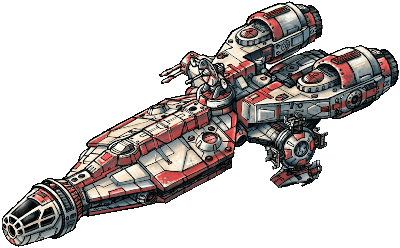
\includegraphics[width=\linewidth]{_img/nimbus.png}
    \caption{Cargo léger YZ-775}
\end{figure}

\paragraph{Background}
Le \textbf{Nimbus} est un cargo léger type YZ-775 modifié par l’alliance rebelle. 52~m de long, 8 membres d’équipage, 12 passagers, 400 tonnes da charge utile. Côté armement il dispose de 1 canon turbolaser double, 2 canons-laser doubles, 2 lance-torpilles à proton.

Il appartient initialement à \nameref{sec:tinon-dystra} qui s’en est servi pour infiltrer le \nameref{sec:pelican} lors d’une mission pour l’alliance. Malheureusement, il ne s’en est pas tiré et le Nimbus est resté à quai sur le Pelican. D’où il a servi de nacelle de secours aux héros.

\paragraph{Traits}

\begin{itemtable}[ c c c c ]
    \textbf{Size} & \textbf{Acc/VMax} & \textbf{Climb} & \textbf{Rés.} \\
    50m           & 45/600            & 1              & 25 (6)       
\end{itemtable}

\paragraph{Défense / Attaque}
\begin{itemtable}[ X c c ]
    \textbf{Arme}     & \textbf{Portée} & \textbf{Dégats}       \\
    Turbo Laser*      & 600             & 4d12                  \\
    Canon Laser (x2)  & 600             & 3d10
\end{itemtable}
* Les Turbolasers sont peu approprié aux vaisseaux rapides comme les chasseurs. Sur un vaisseau dont l’accélération est >= 45, la difficulté de visé est augmenté de +2.